% Options for packages loaded elsewhere
\PassOptionsToPackage{unicode}{hyperref}
\PassOptionsToPackage{hyphens}{url}
%
\documentclass[
]{article}
\usepackage{amsmath,amssymb}
\usepackage{iftex}
\ifPDFTeX
  \usepackage[T1]{fontenc}
  \usepackage[utf8]{inputenc}
  \usepackage{textcomp} % provide euro and other symbols
\else % if luatex or xetex
  \usepackage{unicode-math} % this also loads fontspec
  \defaultfontfeatures{Scale=MatchLowercase}
  \defaultfontfeatures[\rmfamily]{Ligatures=TeX,Scale=1}
\fi
\usepackage{lmodern}
\ifPDFTeX\else
  % xetex/luatex font selection
\fi
% Use upquote if available, for straight quotes in verbatim environments
\IfFileExists{upquote.sty}{\usepackage{upquote}}{}
\IfFileExists{microtype.sty}{% use microtype if available
  \usepackage[]{microtype}
  \UseMicrotypeSet[protrusion]{basicmath} % disable protrusion for tt fonts
}{}
\makeatletter
\@ifundefined{KOMAClassName}{% if non-KOMA class
  \IfFileExists{parskip.sty}{%
    \usepackage{parskip}
  }{% else
    \setlength{\parindent}{0pt}
    \setlength{\parskip}{6pt plus 2pt minus 1pt}}
}{% if KOMA class
  \KOMAoptions{parskip=half}}
\makeatother
\usepackage{xcolor}
\usepackage[margin=1in]{geometry}
\usepackage{longtable,booktabs,array}
\usepackage{calc} % for calculating minipage widths
% Correct order of tables after \paragraph or \subparagraph
\usepackage{etoolbox}
\makeatletter
\patchcmd\longtable{\par}{\if@noskipsec\mbox{}\fi\par}{}{}
\makeatother
% Allow footnotes in longtable head/foot
\IfFileExists{footnotehyper.sty}{\usepackage{footnotehyper}}{\usepackage{footnote}}
\makesavenoteenv{longtable}
\usepackage{graphicx}
\makeatletter
\def\maxwidth{\ifdim\Gin@nat@width>\linewidth\linewidth\else\Gin@nat@width\fi}
\def\maxheight{\ifdim\Gin@nat@height>\textheight\textheight\else\Gin@nat@height\fi}
\makeatother
% Scale images if necessary, so that they will not overflow the page
% margins by default, and it is still possible to overwrite the defaults
% using explicit options in \includegraphics[width, height, ...]{}
\setkeys{Gin}{width=\maxwidth,height=\maxheight,keepaspectratio}
% Set default figure placement to htbp
\makeatletter
\def\fps@figure{htbp}
\makeatother
\setlength{\emergencystretch}{3em} % prevent overfull lines
\providecommand{\tightlist}{%
  \setlength{\itemsep}{0pt}\setlength{\parskip}{0pt}}
\setcounter{secnumdepth}{-\maxdimen} % remove section numbering
\ifLuaTeX
  \usepackage{selnolig}  % disable illegal ligatures
\fi
\IfFileExists{bookmark.sty}{\usepackage{bookmark}}{\usepackage{hyperref}}
\IfFileExists{xurl.sty}{\usepackage{xurl}}{} % add URL line breaks if available
\urlstyle{same}
\hypersetup{
  pdftitle={Factors impacting the frequency of use of urban public transport in Grenoble},
  pdfauthor={RACHDI Mustapha \& SAUNIER Florent \& SAADALLAH Malek},
  hidelinks,
  pdfcreator={LaTeX via pandoc}}

\title{\textbf{Factors impacting the frequency of use of urban public
transport in Grenoble}}
\author{RACHDI Mustapha \& SAUNIER Florent \& SAADALLAH Malek}
\date{\textbf{Janvier 2023}}

\begin{document}
\maketitle

\hypertarget{objective}{%
\subsection{Objective}\label{objective}}

This project is based on data collected in 2010 in the Grenoble region.
The study aims to determine the factors influencing the use of public
transportation. To do this, we set our limits as follows: the Mtag
network, which includes buses classified as ``city'' buses (we did not
take into account regional buses such as the Grenoble - Chamrousse bus),
and the tramway network, whose lines have been expanded since 2010.

\newpage

\hypertarget{methodology}{%
\subsection{Methodology}\label{methodology}}

1- Literature examination

2- Data preparation

3- Key variables definition

4- Univariate Bivariate analysis

4- The model (Not completed yet)

\hypertarget{state-of-the-art}{%
\subsection{State of the art}\label{state-of-the-art}}

\hypertarget{resources}{%
\subsubsection{Resources}\label{resources}}

\begin{longtable}[]{@{}
  >{\raggedleft\arraybackslash}p{(\columnwidth - 8\tabcolsep) * \real{0.0175}}
  >{\raggedright\arraybackslash}p{(\columnwidth - 8\tabcolsep) * \real{0.3474}}
  >{\raggedleft\arraybackslash}p{(\columnwidth - 8\tabcolsep) * \real{0.0281}}
  >{\raggedright\arraybackslash}p{(\columnwidth - 8\tabcolsep) * \real{0.4281}}
  >{\raggedright\arraybackslash}p{(\columnwidth - 8\tabcolsep) * \real{0.1789}}@{}}
\toprule\noalign{}
\begin{minipage}[b]{\linewidth}\raggedleft
\#
\end{minipage} & \begin{minipage}[b]{\linewidth}\raggedright
Authors
\end{minipage} & \begin{minipage}[b]{\linewidth}\raggedleft
Year
\end{minipage} & \begin{minipage}[b]{\linewidth}\raggedright
Title
\end{minipage} & \begin{minipage}[b]{\linewidth}\raggedright
Source
\end{minipage} \\
\midrule\noalign{}
\endhead
\bottomrule\noalign{}
\endlastfoot
1 & Paulley, N., Balcombe, R., Mackett, R., Titheridge, H., Preston, J.,
Wardman, M., \ldots{} \& White, P. & 2006 & The demand for public
transport: The effects of fares, quality of service, income and car
ownership. & Transport policy, 13(4), 295-306. \\
2 & Redman, L., Friman, M., Gärling, T., \& Hartig, T. & 2013 & Quality
attributes of public transport that attract car users: A research
review. & Transport policy, 25, 119-127. \\
3 & Zhang, Wang, M., Dong, J., Lu, W., Liu, Y., Ni, A., \& Yu, X. & 2022
& Factors and Mechanism Affecting the Attractiveness of Public
Transport: Macroscopic and Microscopic Perspectives. & Journal of
Advanced Transportation, 2022, 1--16. \\
4 & Raşca, \& Saeed, N. & 2022 & Exploring the factors influencing the
use of public transport by commuters living in networks of small cities
and towns. & Travel, Behaviour \& Society, 28, 249--263. \\
5 & Göransson, \& Andersson, H. & 2023 & Factors that make public
transport systems attractive: a review of travel preferences and travel
mode choices. & European Transport Research Review, 15(1), 32--14. \\
\end{longtable}

\newpage

\hypertarget{state-of-the-art-1}{%
\subsection{State of the art}\label{state-of-the-art-1}}

\hypertarget{key-factors-from-the-literature}{%
\subsubsection{Key factors from the
literature}\label{key-factors-from-the-literature}}

\begin{itemize}
\item
  \textbf{\emph{Socio-Economic Characteristics:}} Factors like age,
  income, and individual's financial situation.
\item
  \textbf{\emph{Spatial Characteristics:}} The percentage of origin and
  destination municipalities located in high-density areas.
\item
  \textbf{\emph{General Mobility:}} Access to a car and the frequency of
  using alternative modes of transport.
\item
  \textbf{\emph{Alternative-Specific Variables:}} Time, cost, comfort,
  and a combination of time and comfort.
\item
  \textbf{\emph{Instrumental Motives:}} Objective level of service
  variables like travel cost, travel time, and frequency of the
  transport service.
\end{itemize}

\hypertarget{database-handling}{%
\subsection{Database Handling}\label{database-handling}}

\begin{itemize}
\item
  30,702 rows
\item
  116 columns: variables \(=> medium-sized\) database
\item
  971,658 missing values : 27.3\% of the data base
\item
  0\% of the rows have all their values
\item
  21\% of the columns have no missing values
\end{itemize}

\newline

The sample includes 5,189 individuals.

\hypertarget{missing-values}{%
\subsection{Missing values}\label{missing-values}}

\includegraphics{Presentation_files/figure-latex/unnamed-chunk-3-1.pdf}

\hypertarget{missing-values-1}{%
\subsection{Missing values}\label{missing-values-1}}

We can establish some criteria with `r':

Ratio of Missing Values per column =
\frac{Number of Missing Values}{Total Number of Values}

\begin{itemize}
\item
  Good: \(r \leq 5%
  \)
\item
  Medium: \(5% < r \leq 20%
  \)
\item
  Bad: \(20% < r \leq 45%
  \)
\item
  Very Bad: \(r > 45%
  \)
\end{itemize}

\hypertarget{project-variables.}{%
\subsection{Project variables.}\label{project-variables.}}

\hypertarget{frecqtcu}{%
\subsubsection{Frecqtcu}\label{frecqtcu}}

Categorical variable of interest (Y) indicating the frequency of public
transportation usage by an individual.\newline 

It takes the following values: \newline

1\textbar{} Daily use of public transportation.

2\textbar{} Use of public transportation at least twice a week.

3\textbar{} Use of public transportation at least twice a month.

4\textbar{} Very rare use of public transportation.

5\textbar{} Non-existent use of public transportation.

\hypertarget{project-variables.-1}{%
\subsection{Project variables.}\label{project-variables.-1}}

\hypertarget{tailmng}{%
\subsubsection{Tailmng}\label{tailmng}}

Variable indicating the number of people in the household.

\hypertarget{permis}{%
\subsubsection{Permis}\label{permis}}

Variable indicating if a driving license.

\hypertarget{project-variables.-2}{%
\subsection{Project variables.}\label{project-variables.-2}}

\hypertarget{car_ownership}{%
\subsubsection{Car\_ownership}\label{car_ownership}}

Variable indicating whether the person making the journey owns a car.

Depends on three variables:

1 \textbar{} VP\_dispo

2 \textbar{} GENRE: type of vehicle used

3 \textbar{} POSSE: Does the person own the car

\hypertarget{creating-the-new-database}{%
\subsection{Creating the new database}\label{creating-the-new-database}}

Reducing the size of the initial data base with putting restrictions and
removing useless variables.

\hypertarget{geographical-restriction}{%
\subsubsection{Geographical
restriction}\label{geographical-restriction}}

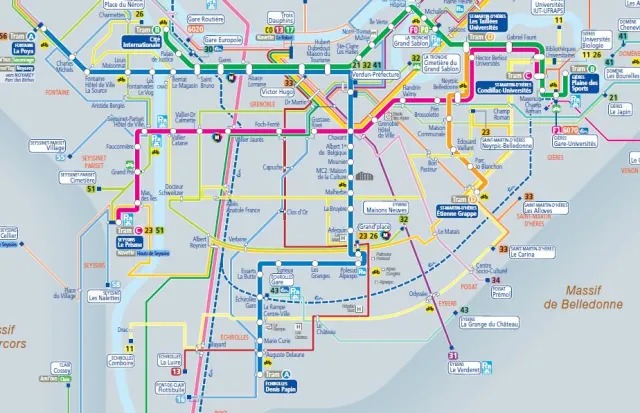
\includegraphics{reseau tag.jpg}

\hypertarget{creating-the-new-database-1}{%
\subsection{Creating the new
database}\label{creating-the-new-database-1}}

\hypertarget{age-restriction}{%
\subsubsection{Age restriction}\label{age-restriction}}

\newline

Removing minors (\textless{} 18 yo) and very old people (\(> 88\) yo)

\includegraphics{Presentation_files/figure-latex/unnamed-chunk-14-1.pdf}

\hypertarget{univariate-analysis}{%
\subsection{Univariate Analysis}\label{univariate-analysis}}

\hypertarget{usage-frequency}{%
\subsubsection{Usage frequency}\label{usage-frequency}}

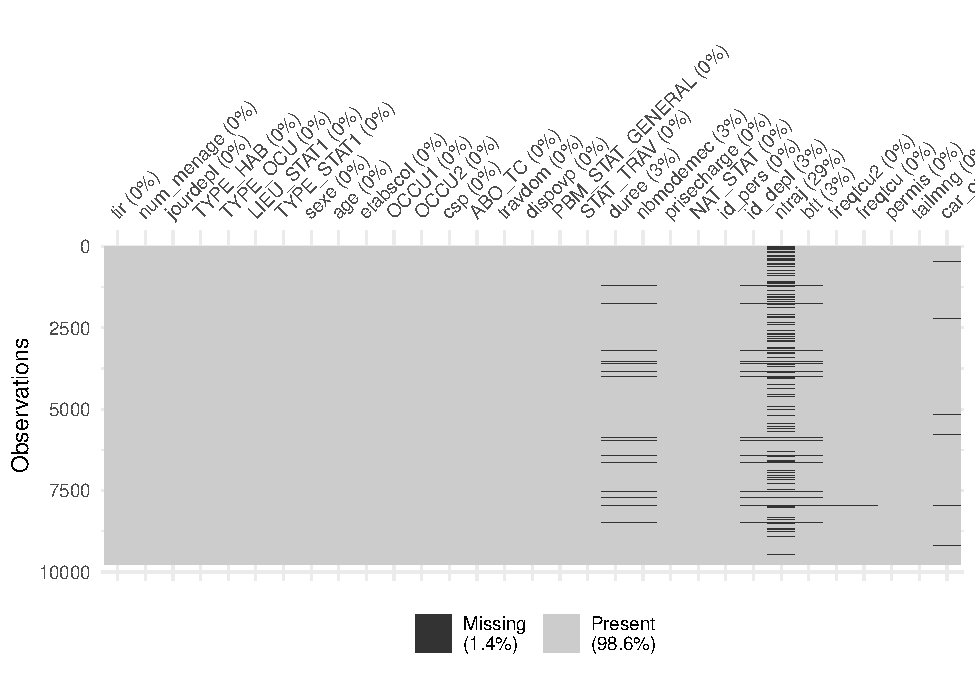
\includegraphics{Presentation_files/figure-latex/unnamed-chunk-15-1.pdf}

\hypertarget{univariate-analysis-1}{%
\subsection{Univariate Analysis}\label{univariate-analysis-1}}

\hypertarget{driving-license}{%
\subsubsection{Driving license}\label{driving-license}}

\textbf{Everyone has a driving license.} \newline

\hypertarget{univariate-analysis-2}{%
\subsection{Univariate Analysis}\label{univariate-analysis-2}}

\hypertarget{household-size}{%
\subsubsection{Household size}\label{household-size}}

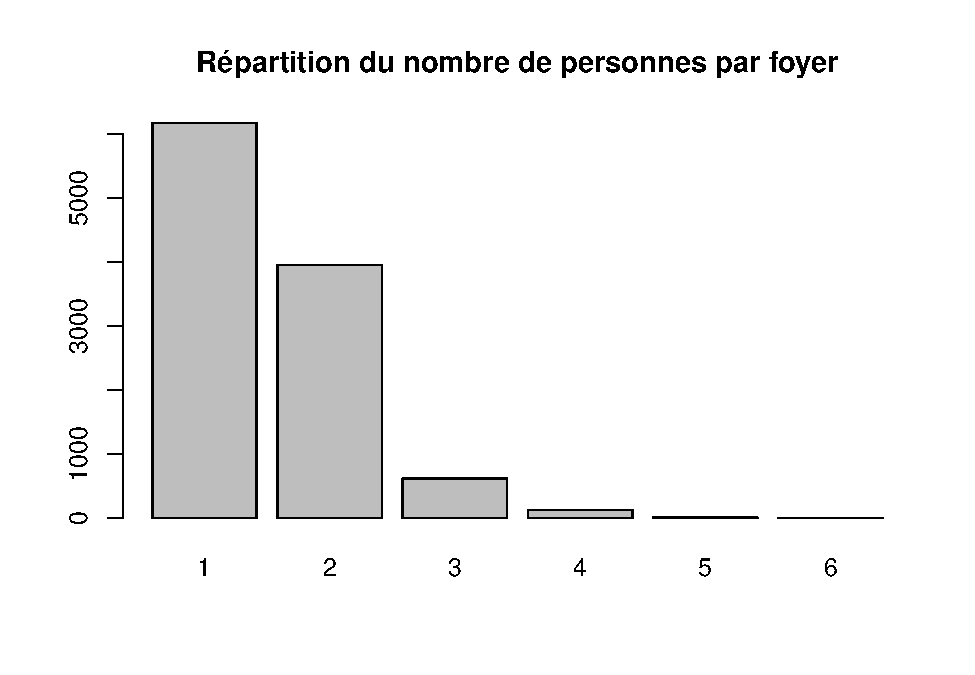
\includegraphics{Presentation_files/figure-latex/unnamed-chunk-17-1.pdf}

\hypertarget{bivariate-analysis}{%
\subsection{Bivariate Analysis}\label{bivariate-analysis}}

\textbf{Chi-squared test} \newline

\begin{longtable}[]{@{}
  >{\raggedright\arraybackslash}p{(\columnwidth - 8\tabcolsep) * \real{0.2353}}
  >{\raggedright\arraybackslash}p{(\columnwidth - 8\tabcolsep) * \real{0.1912}}
  >{\raggedright\arraybackslash}p{(\columnwidth - 8\tabcolsep) * \real{0.1765}}
  >{\raggedright\arraybackslash}p{(\columnwidth - 8\tabcolsep) * \real{0.1618}}
  >{\raggedright\arraybackslash}p{(\columnwidth - 8\tabcolsep) * \real{0.2353}}@{}}
\toprule\noalign{}
\begin{minipage}[b]{\linewidth}\raggedright
Variable
\end{minipage} & \begin{minipage}[b]{\linewidth}\raggedright
Fisher Test
\end{minipage} & \begin{minipage}[b]{\linewidth}\raggedright
Chisq test
\end{minipage} & \begin{minipage}[b]{\linewidth}\raggedright
R squared
\end{minipage} & \begin{minipage}[b]{\linewidth}\raggedright
Significance
\end{minipage} \\
\midrule\noalign{}
\endhead
\bottomrule\noalign{}
\endlastfoot
tailmng & 0.22 & & 0.0021 & Moderate \\
car\_ownership & & 2.2e-16 & & \\
NB\_actif & 0.002 & & 0.0016 & No significant \\
NB\_inactif & 0.00039 & & 0.006 & High significant \\
NB\_retraites & 0.000498 & & 0.01437 & High significant \\
NB\_etu & 0.000498 & & 0.04654 & High significant \\
NB\_log\_ind & 0.000498 & & 0.04991 & High significant \\
NB\_proprietaire & 0.000498 & & 0.01648 & High significant \\
NB\_locataire & 0.000498 & & 0.068 & High significant \\
NB\_log\_col & 0.000498 & & 0.08347 & High significant \\
NB\_stat\_parking & 0.000498 & & 0.0059 & High significant \\
NB\_stat\_garage & 0.000498 & & 0.0065 & High significant \\
NB\_stat\_rue & 0.000498 & & 0.004081 & significant \\
NB\_stat\_interdit & 0.000498 & & 0.002658 & significant \\
\end{longtable}

\hypertarget{whats-next}{%
\section{What's next ?}\label{whats-next}}

\end{document}
